\section{Optimized single neurons}
In the previous sections we saw that optimization of models to the mean features reported across many neurons, even of the same nominal type, is conceptually and empirically flawed.
The remainder of the optimization results will focus instead on the optimization of single neurons.
In other words, I will produce optimized models that used only features extracted from recordings of the same neuron, and those models will putatively represent any neuron that behaves as that one did.
This conveniently eliminates not only variability across neurons of the same type, but also variability across recordings sessions or labs, since by experimental necessity intracellular recordings are collected in a matter of minutes in a single lab.

Table \ref{tab:single-neuron-constraints} which constraints (i.e. NeuronUnit tests were used to guide this process.  
These constaints were different from those used in the NeuronUnit tests for two reasons: a) NeuronUnit contains very little data about some of these features and b) the single neuron data used here was collected using a family of suprathreshold stimuli that allow many complex spike-pattern features to be calculated.

%%%
% Note to self, 
% Table and caption represents an older approach. What is written is true, for the time that it was used, but it no longer reflects the features mainly used to guide optimization
%%%
\begin{table}[]
    \centering
    \resizebox{1\textwidth}{!}{
    \begin{tabular}{c|c|c}
    \toprule
Feature Name & Description \\
adaptation-index & Adaption Index for above $0mV$ spikes \\
adaptation-index2 & Adaption Index for a mixture of above and below $0mV$ spikes \\
time-to-first-spike & The time in seconds to first spike \\
mean-AP-amplitude & The average in AP amplitude \\
spike-half-width & Spike width measured at half amplitude \\ 
AHP-depth & After Hyperpolarization Depth \\ 
minimum-voltage & Minimum voltage in $V_{M} $ recording \\
peak-voltage & Peak voltage in $V_{M}$  recording \\
time-to-last-spike & Time elapsed until final spike. \\
AHP-depth-abs & Mean after-hyperpolarization amplitude. \\
all-ISI-values & All Inter Spike Interval Values \\
voltage-base & The base voltage of $V_{M}$ while undergoing stimulus. Often not the minimum $V_{M}$ \\
min-voltage-between-spikes & The minimum voltage between spike in $V_{M}$, while neuron undergoing stimulus \\
Spikecount & Number of spikes observed in model, given appropriate AP \\
\bottomrule
    \end{tabular}}
    \caption[Constraints for Suprathreshold Single Neuron Model Fits]{A table of constraints that were used to guide single neuron optimization using suprathreshold stimuli.
    This set varied across optimizations, depending on which underlying stimuli were available in the recorded experimental data.
    While features such as AHP depth and Minimum Voltage between spikes improved optimization, all things being equal, if they were given too much priority (over statistics derived from spike times or amplitudes) then fit quality was reduced.}
    \label{tab:single-neuron-constraints}
\end{table}

% \end{verbatim}

%\begin{table}[]
%    \centering
%    \resizebox{1\textwidth}{!}{
%    \begin{tabular}{c|c|c}
%    \toprule
%        Feature Name & Description & injection strength \\
%        AHP-depth-abs & After Hyperpolarisation Depth absolute value & $3.0 \times $ Rheobase \\ 
%        sag-ratio2 & Difference between maximum negative deflection of $V_{M}$ and steady state $V_{M}$ during negative stimulus application &  $3.0 \times $ Rheobase \\ Input Resistance $\frac{V_{M}}/{I_{stimulus}}M \Omega$ &  $1.5 \times $ Rheobase \\ 
%        peak-voltage & time of peak voltage &  $3.0 \times $ Rheobase \\
%        voltage-base & value of base voltage (minimum $V_{M}$ during stimulus &  $3.0 \times $ Rheobase \\
%        Spikecount & Number of spikes during stimulus &  $3.0 \times $ Rheobase  \\
%        ohmic-input-resistance-vb-ssse & Input Resistance from voltage base steady state equilibrium &  $1.5 \times $ Rheobase  \\
%    \bottomrule
%    \end{tabular}}
%    \caption[Constraints for Suprathreshold Single Neuron Model Fits]{A table of constraints that were used to guide single neuron optimization using suprathreshold stimuli.
%    This set varied across optimizations, depending on which underlying stimuli were available in the recorded experimental data.
%    While features such as AHP depth and Minimum Voltage between spikes improved optimization, all things being equal, if they were given too much priority (over statistics derived from spike times or amplitudes) then fit quality was reduced.}
%    \label{tab:single-neuron-constraints}
%\end{table}

\subsection{Optimization of Blue Brain Project Neurons}
I use two data sources for these results.
First, I use a somatic current injections conducted on a rat somato-sensory hind limb neurons as part of the Blue Brain Project.

Figure \ref{fig:B95Adexp} shows an example of an AdEx model optimized against data from such a neuron, which provided a challenging response (to somatic current injection) to fit.
For example, while spike rate adaptation can be observed in this neuron, it is not monotonic: while the inter-spike-intervals (ISIs) are generally increasing, the final ISI is actually slightly shorter than the penultimate one.
Nonetheless, the optimizer achieves a reasonably good match to this pattern of spikes, as well as to the resting potential and the spike threshold.
It performs less well at capturing the hyperpolarization between spikes.
Similar results are shown using an Izhikevich model (Figure \ref{fig:B95_IZHI}).
The AdEx model is somewhat better at matching spike times than the Izhikevich model, consistent with the literature \cite{rossant2011fitting}. 

\begin{figure}
    \centering
    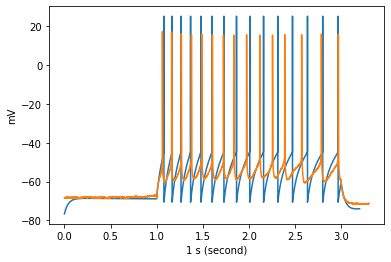
\includegraphics[scale=0.75]{figures/bbp_multispiking_fit.png}
    \caption[Optimized AdEx model from BBP]{An Adaptive Exponential (AdEx) model was optimized to both the spike times and shapes from a single neuron in the Blue Brain Project Microcircuit Portal data (taken from animal ID B95)
    %\url{http://microcircuits.epfl.ch/#/animal/8ecde7d1-b2d2-11e4-b949-6003088da632}
    While there as some ``misses" in the subthreshold behavior in between spikes, and in the amplitudes of the spikes, the basic pattern of spiking is successfully recapitulated.}
    \label{fig:B95Adexp}
\end{figure}

\begin{figure}
    \centering
    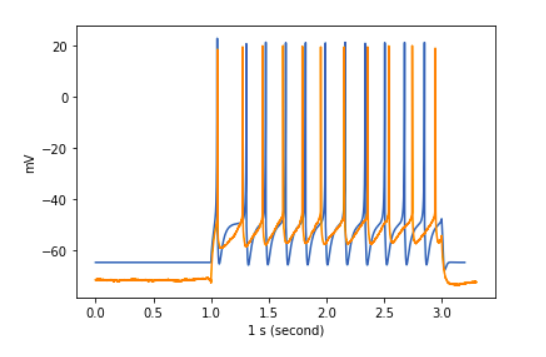
\includegraphics{figures/IZHI_B95.png}
    \caption[Optimized Izhikevich model from BBP]{Similar to Fig. \ref{fig:B95Adexp}, but instead using an Izhikevich model.
    Here optimisation is a bit worse, but not poorer than the best out-of-sample predictions of spike timing from previous efforts.}
    \label{fig:B95_IZHI}
\end{figure}

\subsection{Allen Cell Types Database Neurons}
I then used similar data for mouse neurons taken from primary visual cortex and optimized the AdEx model (which gave the best results for the BBP data considered above).
These results were improved over those using the BBP neuron data.
As shown in Figures \ref{fig:specimen_476053392_A}, \ref{fig:specimen_476053392_B} and \ref{fig:specimen_325479788}, optimized models of this flavor were capable of reproducing patterns of spikes and (to a better extent than using the BBP data) subthreshold dynamics.
The same optimized model was also capable of reproducing the patterns of spikes in response to different amplitudes of somatic current injection (Figs \ref{fig:specimen_476053392_A} and \ref{fig:specimen_476053392_B}).

\begin{figure}
    \centering
    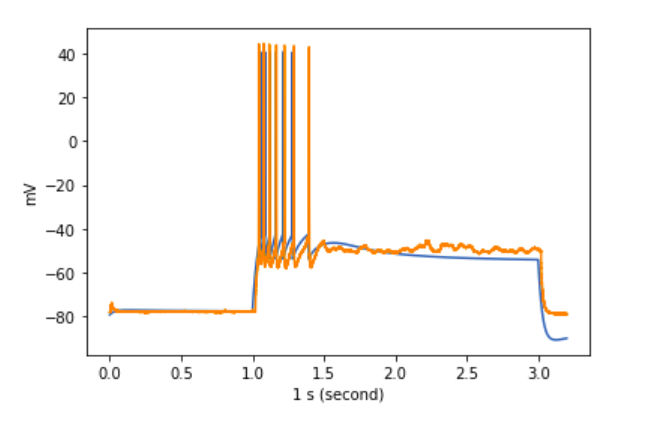
\includegraphics[scale=1]{figures/adexp_fit_allen_spec_id_476053392.png}
    \caption[Optimized AdEx model from Allen Cell Types (A)]{An adaptive Exponential Model was fitted to both the spike time, and spike shape data in a sweep from Allen specimin id: 476053392}
    \label{fig:specimen_476053392_A}
\end{figure}

\begin{figure}
    \centering
    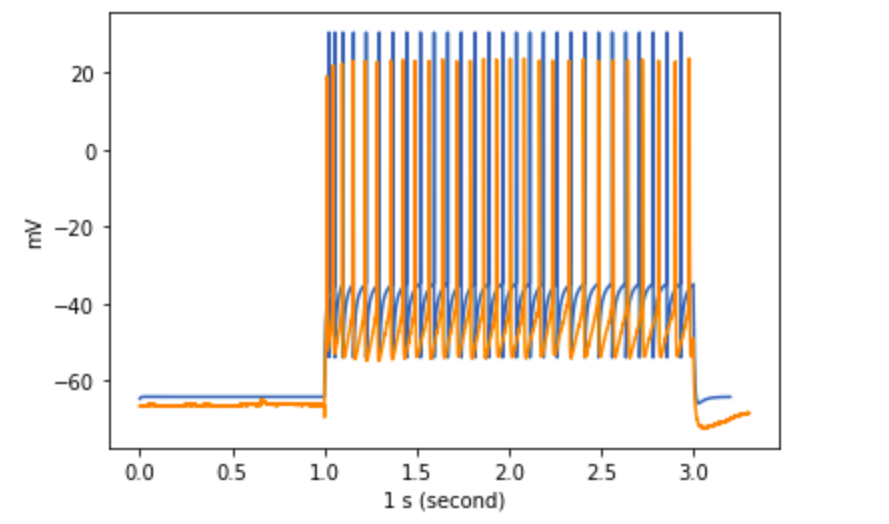
\includegraphics[scale=1]{figures/28spikesB95}
    \caption[Optimized AdEx model from Allen Cell Types (B)]{An adaptive Exponential Model was fitted to both the spike time, and spike shape data in a sweep from Allen specimin id: 476053392}
    \label{fig:specimen_476053392_B}
\end{figure}

%Similar to Druckmann Suprathreshold depolarizing step currents \cite{druckmann2008evaluating}.
\begin{figure}
    \centering
    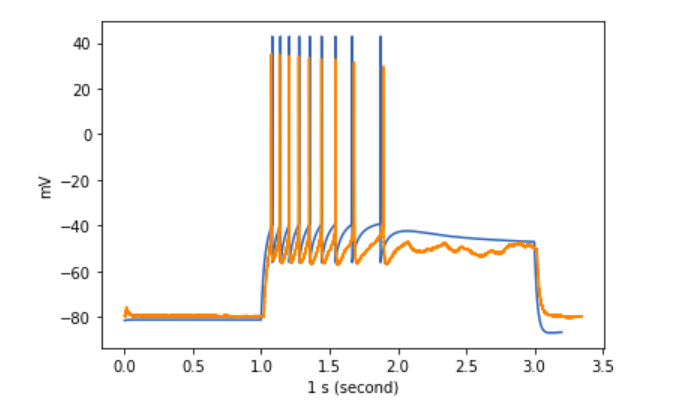
\includegraphics[scale=1]{figures/adexp_fit_allen_specid_325479788.png}
    \caption[Optimized AdEx model from Allen Cell Types (C)]{ An adaptive Exponential Model was fitted to both the spike time, and spike shape data in a sweep from Allen specimin id: 325479788}
    \label{fig:specimen_325479788}
\end{figure}

\subsection{Comparison to Best-Case Scenarios}
Since these result now concern fits to single neurons, I cannot use the $\chi^2$ measure of agreement between the optimized model and the distribution of the data; the distribution now has only a single member per optimization.
Instead, I will compare the quality of these results to best-cases scenarios from prior research.
I will also use the ``variance explained ratio" between the allen institute experimental sweep and the optimized models sweep to a comparable current injection.

Previously, a competition was held \citep{naud} inviting participants to predict spike times (in response to specific patterns of somatic current injection) for well-characterized cortical neuron.
The best models in this competition were only able to predict $\sim86\%$ of spike times (Fig. \ref{fig:rossant-fits}), and this under conditions with fluctuating somatic currents that actually produce more spike-timing regularity than square currents \citep{mainen}.
Consequently, it is unlikely that \emph{in silico} models can be expected to produce a perfect match of spike times in response to square wave current injection, tempering expectations for my optimizer.
As noted in the previous optimization efforts \citep{druckmann2007novel}, it is probably mistaken to fit models to precise spike times; real cortical neurons produce and receive noisy currents, and likely rarely exhibit identical spike trains even in response to the same nominal stimulus.
Optimization on derived features of spike timing and rate, such as statistics of distributions of ISIs, of F-I curves, is a more promising approach.

\begin{figure}
    \centering
    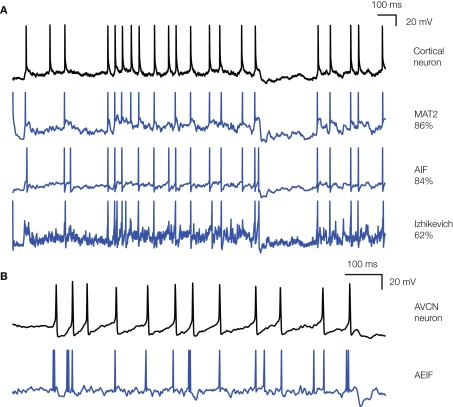
\includegraphics[scale=5.0]{figures/IZHIkevich_fit_60Adexp_80.jpg}
    \caption[Model Fits in Prior Work]{This figure from  \cite{rossant2011fitting} shows how the majority of models that fit spike time, do not also fit spike shape. Spike shape and AP timing constitute a persistent conflicted priority with regards to model fitting. Included in this figure are fits from reduced models used in this work. Including the Izhikevich model, and the AIF model (herein referred to as AdEx). In this  context the MAT2 model correctly predicts $86$ of spike times, but you can see that the spike threshold is much higher in the model compared to the experiment. The Izhikevich model only predicts $62\%$ of spike times (this is also consistent with my results), and it displays much more below threshold activity than the data and the other models.} 
    \label{fig:rossant-fits}
\end{figure}

%\begin{comment}
%\begin{figure}
%    \centering
%    \begin{subfigure}[t]
%        \centering
%        \includegraphics[width=0.5\linewidth]{example-image-a.pdf} 
%        \caption{Generic} \label{fig:timing1}
%    \end{subfigure}
%    \hfill
%    \begin{subfigure}[t]
%        \centering
%        \includegraphics[width=0.5\linewidth]{example-image-b.pdf} 
%        \caption{Competitors} \label{fig:timing2}
%    \end{subfigure}
%
%    \vspace{1cm}
%    \begin{subfigure}[t]
%        \centering
%        \includegraphics[width=0.5\linewidth]{example-image-c.pdf} 
%        \caption{Price regulation} \label{fig:timing3}
%    \end{subfigure}
%    \hfill
%    %\begin{subfigure}[t]%{0.45\textwidth}
%    %    % just an empty subfigure to shift C below A
%    %\end{subfigure}
%    \caption{Some general caption of all the figures. In (\subref{fig:timing1}) %you can see a  green square....}
%\end{figure}
%\end{comment}

% TODO make multi panel.




% Interesting direct qoute from Druckmann:
%"In experiments, intrinsic noise gives rise to a large variability (e.g., in firing pattern) in the voltage responses to repetitions of the exact same input. Thus, the common approach of fitting models by attempting to perfectly replicate, point by point, a single chosen trace out of the spectrum of variable responses does not seem to do justice to the data."

%In experiments, however, when the exactly same stimulus is repeated several times, the voltage traces elicited differ among themselves to a significant degree (Mainen and Sejnowski, 1995; Nowak et al., 1997).








